\documentclass[11pt]{article}
\usepackage{graphicx}
\usepackage{hyperref}
\begin{document}
\title{ CS7038: Group Project\\School of Computer Science and Statistics\vspace{0.6cm}\\Trinity College Dublin\vspace{0.4cm}\\
\includegraphics[scale=1.5]{TCD.jpg}\vspace{0.6cm}\\Final Report}
\author{Yafie Qu, Hao Guan, Jeremiah Dunn, Saloni Sharma}
\maketitle
\section{Overview of the Project}
\subsection{Story}
Our game takes place on a spaceship which is on a long journey. The ship's computer begins malfunctioning, different subsystems start failing and the security system begins to malfunction. The crew of the ship is in stasis and unaware of the situation. The player  character, the maintenance droid is the only unaffected robot or computer on the ship. His task is to restore power to ship's subsystem while avoiding the security system. The ship's fate is in the hands of this humble maintenance droid.
\subsection{Theme}
This is the International Year of Light and Light-based Technologies. This is a United Nations observance that aims to raise awareness of the achievements of light science and its applications and importance.\\

Our game incorporates light as one of the main mechanics for exploring the ship. When the space ship is wrecked and malfunctions, it looses all its power sources and light. The player character returns power to the ship, gradually lighting it up in the process. Restoring light makes the ship easier to navigate and directs the player towards the exit of each level.\\

\subsection{Initial Design}
The game is an exploration based 2D platformer similar to games like \textit{Spelunker}. It is designed to be played using the Unity web-player. The initial design was focused on randomised level generation. Using this a large variety of different looking levels can be created from a handful of prefabs.

The gameplay is influenced by the dynamic lighting system which changes the appearance of the ship. These dynamic lighting effects are generated by the placement of point and spot lights and use if normal maps for different game objects.

\section{Technical Overview}
The game is made using \textit{Unity}. Game physics are implemented using Unity 2D physics engine. Normal maps and height maps are created with the assistance of \textit{SpriteLamp} and \textit{Crazy Bump}.

\subsection{Level Generation}
Each level begins as 2D grid of an arbitrary size. A \textit{solution path} is then generated through the level as shown in figure \ref{Fig:Data1}. First a point on the top of the grid is randomly picked as the start of the level. We then can step through the grid towards the bottom. Now a left/right is chosen randomly. There is then a random chance of stepping in this direction or stepping down. After stepping down, we chose our random direction again and repeat the process. When we reach the bottom floor the probability of going down is replaced by a probability of choosing the exit.\\

We then assign different room types to each point on the \textit{solution path}. These room types correspond to the exits/entrances that each room needs. After this, we draw a boundary around the level. Doing this minimises the amount of different exit types we need to design to the four shown in figure~\ref{Fig:Data2}.

\begin{figure}[!htb]\centering
   \begin{minipage}{0.49\textwidth}
     \frame{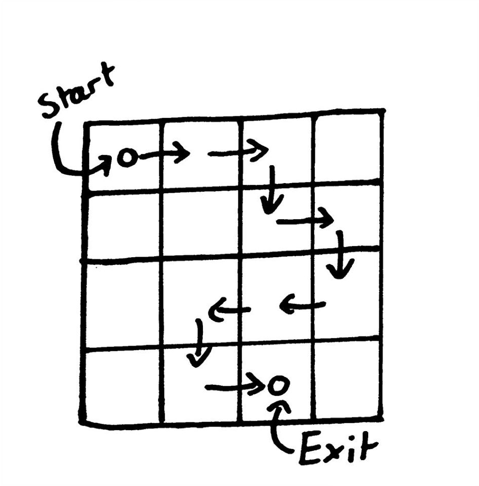
\includegraphics[width=\linewidth]{levelgen1.png}}
     \caption{Solution Path Generation}\label{Fig:Data1}
   \end{minipage}
   \begin {minipage}{0.49\textwidth}
     \frame{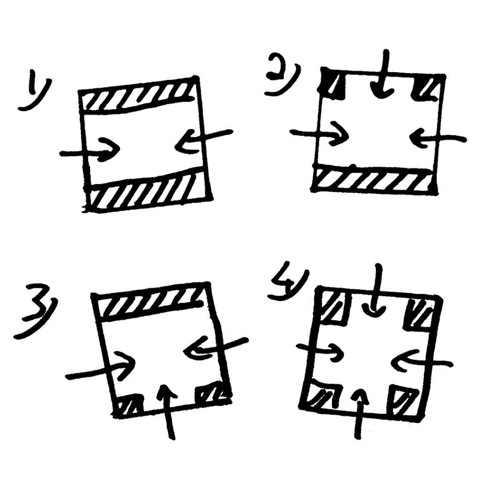
\includegraphics[width=\linewidth]{levelgen2.png}}
     \caption{Room Types}\label{Fig:Data2}
   \end{minipage}
\end{figure}

\subsection{Rooms}
Rooms are 16x16 grids of tiles, there are different rooms for the different exit types. Rooms are represented by \textit{CSV} text files an example of which can be seen in figure~\ref{Fig:Data3}. In the text files, different characters are used as identifiers for different tile types. For example \textit{G} represents a solid, walk-able surface, while \textit{T} represents a trap tile. Modifiers to the tiles, such as the radius of a light, can be added after the identifier. These can be easily swapped out of the game to create and test new levels.\\


\begin{figure}[!htb]\centering
   \begin{minipage}{0.49\textwidth}
     \frame{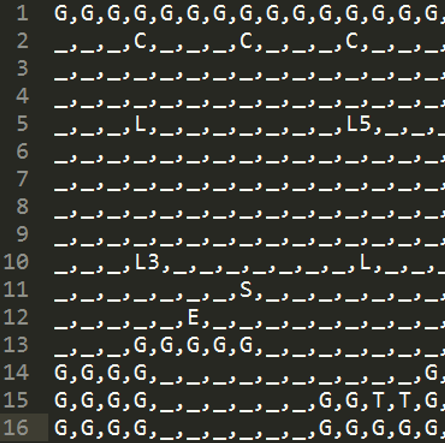
\includegraphics[width=\linewidth]{room.png}}
     \caption{Input text file}\label{Fig:Data3}
   \end{minipage}
   \begin {minipage}{0.49\textwidth}
     \frame{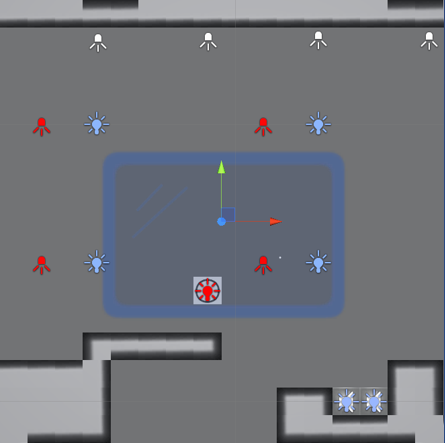
\includegraphics[width=\linewidth]{room1.png}}
     \caption{Unity Editor Output}\label{Fig:Data4}
   \end{minipage}
\end{figure}

\subsection{Lighting System}
To follow the theme of light, the game uses light to change the appearance of the level as game progresses. Unity gives the privilege to use 3 types of lights in the free version. The game uses two of these different lights which can be placed in the room using input comma separated text files. Text files can also take the light radius as an input.\\

The first type of light is the spot light which is used for general illumination and ambience. The second type of light is the point light which is used to light specific areas. The lighting system has greater visual impact on the scene. The game also handles the tweaking in of ambient light level when the player is in different room. To create light effect on the game objects around a light source, normal mapped sprites are being used.
\subsection{Security System}
Since the space ship's security system is malfunctioning, the game-play implemented in a way to have defence measures and show this unusual behaviour of security system using different components such as  electric traps, alarm and security droid/enemy.\\

The security system can be tripped when our robot re-activates components of the ship. When the ship enters an alarm state, the security droid and electric traps are activated. The security droid chases the maintenance droid(our Player robot) and drains his energy. The trap tiles shock the player robot with an electric bolt. The robot can deactivate the alarm by interfacing with another component.
\subsection{Player Character}
The player controls the character directly as a traditional 2D platformer. The game-play includes the energy system for the player. The energy also drains as the time goes which means the player has to speed up to complete the level. When activating the ship's components the player can recharge a portion of its energy. This also motivates the player to explore the ship and complete the level.\\

The camera is dragged along by the player and moves in 3-dimensional space. There are two lights attached to the player game object. The spot light attached is used to handle the navigation torch light in a dark room. The other is the point light is used to make the eye of the robot visible. The normal mapped sprites are used for the player character with bump mapping to add the depth to the scene which is visible when camera pans.
\section{Team Organisation}
Scrum has been used for the product development which is an iterative and incremental agile software development methodology for managing product development.\\

The team has used Jira for project management and Git as a repository for synchronised progress across team and for  maintaining development using stable branches.\\

The team created high level overview of tasks called as Epics. The game project idea is divided into these Epics: \textit{Level Generation}, \textit{GUI}, \textit{Core Game} and \textit{Character Controller}.\\

These Epics were further broke down into smaller and manageable tasks called as Stories. The project was divided into 4 sprints. Each sprint lasted for 2 weeks. At start of each sprint, team had regular grooming sessions to estimate and re-estimate the stories and their implementation time. Task for each sprint will be chosen from the backlog based on their priority and requirements. In the grooming sessions, team looked through the backlog and see what stories they want to work on, assign story points, give them time estimates and flesh-out the descriptions or sub-task them as required. Time estimation for different tasks has been carried off by using voting system and then taking average of individual estimated time.\\

Team had regular stand-ups, an average of thrice a week. Stand-ups were aimed to last for 10 minutes with any additional discussions happened in separate meeting outside this time. The team had a different scrum master for each sprint from one of the team members.\\

Team prioritized the project stories by keeping Level generation and core game on high priority and GUI on the least priority. This was implemented for an organized way of development so that major game-play could be implemented on time keeping an account of time spent on other assignments of coursework. During the course of project, team learned more about Unity and skills/efficiency of different team members.

\section{Conclusion}
The team has implemented almost all the tasks they have aimed for. Starting for the level generation with file handler to game logic implementation to GUI. Team also worked dynamically to add new features to make the game-play interesting for the player by adding enemy droid and the player energy system. Team showed good organizational skills to achieve its goals. The project has been successfully implemented the scrum methodology.\\

There are also certain functionalities which could have been used as a library for future projects. One of them is Level Editor. A randomised level generation has been implemented which takes input from csv files which is also scalable. This implementation could be extended to make a standalone library for level editor in Unity.
\section{You Tube Link}

\section{Acknowledgements}
We would like to express our very great appreciation to Dr. John Dingliana for his valuable and constructive suggestions during the planning and development of this game. We would also like to acknowledge our friend Ting Zhang for her ideas for the asset creation and to work in collaboration with the whole team.  
\end{document}